%!TEX root = ../../prace.tex

\section{Struktura projektu v~Unreal Engine TODO}
\label{sec:ueStructure}

Nejzákladnějším prvkem celého projektu v~\UEu{} jsou herní \textit{mapy}. Mapy obsahují herní objekty, které tvoří jádro hry. Mohou to být viditelné (renderovatelné) objekty, ale i~různé objekty implementující herní logiku. Těm druhým se obvykle říká \textit{kontroléry}, protože nedělají nic jiného, než jen nějakým implementovaným způsobem řídí hru.

Všechny herní objekty, které lze v~Editoru použít, je možné najít ve \textit{Správci obsahu}. Ten má mj.~složku \textit{Content}, jejíž obsah odpovídá stejnojmenné složce z~hlavního adresáře hry, a~složku \textit{C++ Classes}, která odpovídá programové struktuře ze složky \textit{Source} v~hlavním adresáři hry. Pojďme si nyní popsat hlavní části hry.


\subsection{Mapy}

V naší hře máme 4 mapy a~to:

\begin{itemize}
	\item GameLoader -- tato mapa je nastavena jako výchozí po spuštění hry. Má na starost počáteční konfiguraci nastavení hry, například aplikaci nastavení jazykové mutace. Po dokončení všech inicializačních akcí hra pokračuje načtením mapy \textit{MainMenu}.
	\item MainMenu -- tato mapa slouží čistě pro účely zobrazení hlavního menu hry. Obsahuje v~sobě mapu \textit{MainMap}, což je z~toho důvodu, že jsme chtěli v~hlavním menu zobrazovat herní svět. Ten si, umělecky řečeno, \uv{žije svým vlastním životem}. Z~hlavního menu tedy můžeme pozorovat průběh denního cyklu, nebo změny počasí.
	\item LoadingScreen -- tato mapa má na starosti nahrávání hry. Za použití streamování hlavní herní mapy je možné renderovat průběh načítání hry a~zobrazovat případné další hlášky o~stavu nahrávání.
	\item MainMap -- pro nás nejdůležitější mapa, obsahuje veškerou naši herní logiku. Proto se na ni podrobněji zaměříme.
\end{itemize}

\subsection{Hlavní herní mapa}

Hlavní struktura objektů v~rámci herní mapy je vidět na obrázku \ref{fig:ue_mainMap}. Nás budou nejvíce zajímat objekty \textit{WorldController}, \textit{SkyBP}, \textit{GameElectricityPawn},\linebreak a~\textit{GameWeatherPawn}. Těm se budeme věnovat podrobněji v~následující části práce.

U zbývajících stojí za zmínku pouze \textit{Landscape6}, který na sobě má Tag, díky kterému tento herní objekt nebudeme ignorovat v~rámci výpočtů míření hráče na bloky. Kdyby to bylo možné, přiřadili bychom objektu terénu komponentu cíle zaměřování (stejně jako u~bloků), nicméně v~současné době \UE{} tuto funkcionalitu nenabízí.

\begin{figure}[!ht]\centering
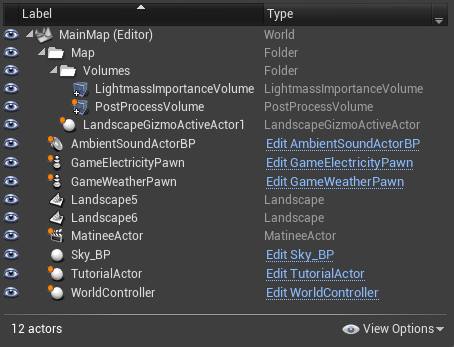
\includegraphics[ width=100mm]{../img/program/mainMap}
\caption{Přehled objektů hlavní mapy}
\label{fig:ue_mainMap}
\end{figure}
\FloatBarrier


\subsubsection{Průběh nahrávání hlavní herní mapy}

Jakmile je vyvolána událost \textit{BeginPlay}, hra se podívá do hlavní herní instance\footnote{Herní instance je jediná třída v~\UEu{}, která je stejná po celou dobu života hry. V~zásadě tak kopíruje koncept návrhového vzoru \textit{Singleton} a~my ji můžeme využít pro předávání informací při přechodu mezi mapami.}, jaký level je požadován na nahrání. Tato informace je do herní instance uložena během výběru nové hry, či v~případě hlavního menu z~hlavního Blueprintu mapy. Protože nemáme zajištěné pořadí vykonávání události \textit{BeginPlay}, musíme počkat, než nám některé objekty (jako třeba WorldController) dají najevo, že byly úspěšně inicializovány.

Další logika je snadná -- proběhne pokus o~kompletní načtení dat do instance objektu uložené hry a~postupně u~všech herních objektů s~podporou ukládání her voláme načítání dat z~objektu uložené hry. Po ukončení této fáze se hra pokusí zobrazit případné chyby vzniklé během načítání (což nejčastěji bude spíše validační hláška) a~vyvolá se odtemnění skrze \textit{Remote Event}. Na tuto událost pak reaguje mapa LoadingScreen (jež načítání MainMap vždy vyvolá) a~proběhne animace, kdy se nahrávací obrazovka postupně zprůhlední, až nakonec není vidět.


\subsection{World Controller}

\textit{World Controller} je především implementován v~\CPP{}. Ačkoliv je v~hlavní herní mapě umístěn jeho Blueprintový potomek, ten sám nepřináší nic významného. Cílem tohoto kontroléru je správa bloků v~herním světě a~všeho, co se toho týká.

Tento herní objekt si udržuje seznam všech herních bloků v~herním světě. Zároveň má ke každému bloku dynamicky přiřazenou obsluhu různých událostí. Společnou pro všechny je \TT{OnDestroyRequestedEvent}, která je definovaná v~bázové třídě bloků a~slouží k~notifikaci toho, že se blok chce zničit. Tato událost může být vyvolána jako důsledek kyselého deště, kdy po zásazích kleslo zdraví bloku na nulu.

Další důležitou vlastností tohoto objektu je držení reference na kořen stromové struktury reprezentující umístění bloků v~herním světě. Této vlastnosti pak mohou využívat ostatní objekty hry a~kupříkladu se mohou dotazovat na volné místo.


\subsection{bloky}

Kde a~jak definované, obrázek, jak se to definuje konstanty


\subsection{GameElectricityPawn}

Herní objekt GameElectricityPawn má přiřazenou komponentu\linebreak \TT{UGameElectricityComponent}, která spravuje všechny elektrické sítě v~herním světě. \textit{World Controller} si během události \textit{BeginPlay} tento herní objekt najde a~uloží si referenci na komponentu správy elektrických sítí. Díky tomu poté může bloky přidávat či odebírat ze sítě voláním příslušných metod v~elektrické komponentě.


\subsection{GameWeatherPawn}
GameWeatherPawn funguje jako správce počasí. Je ovládán \textit{AI kontrolérem}, který je možné nalézt v~\TT{/Content/Blueprints/World/Weather}. V~té samé složce je možné nalézt všechny assety, které s~počasím souvisí. Mimo jiné je zde možné nalézt ovládací Behavior Tree. Podoba ovládacího behaviorálního stromu je vidět na obrázku \ref{fig:weatherBP}. Strom se v~zásadě nijak neliší od uvažovaného automatu z~kapitoly (TODO ref!). 

Služba aktualizace času (na obrázku zeleně) neustále aktualizuje uplynulý herní čas a~řídí se přitom hodnotou z~(todo ref) herního objektu oblohy. Dále máme ve stromě tři funkce, které se starají o~kontrolu stavu počasí a~případnou aktualizaci navázaných herních objektů -- oblohy. 

Oproti automatu jsme zde přidali drobnou optimalizaci -- pokud jsme ve fázi stabilního počasí a~neměníme žádné parametry, vyhodnocování stromu přejde do nejpravější větve, kde bude čekat po nějaký spočítaný čas. Spolu s~vhodným nastavením aktualizační služby jsme tak dosáhli toho, že během této doby jsou aktualizace méně časté (protože je stejně k~ničemu nepotřebujeme a~ušetříme tak výpočetní čas), ale jakmile se mění počasí, aktualizace uplynulého času je častější.


\begin{figure}[!ht]\centering
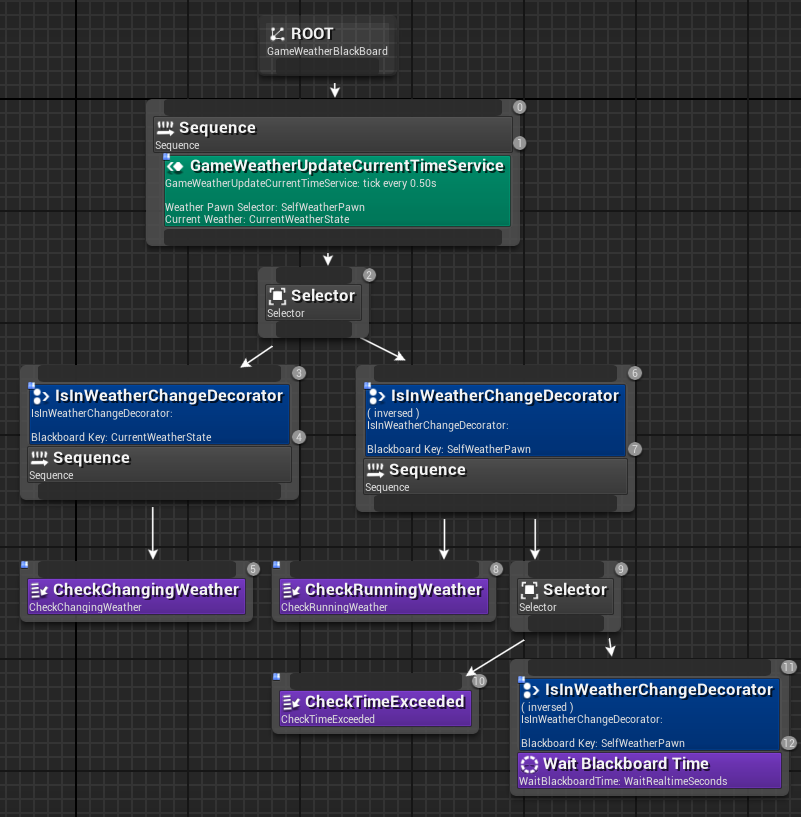
\includegraphics[ width=140mm]{../img/program/weatherBT}
\caption{Behavior Tree pro ovládání počasí}
\label{fig:ue_weatherBP}
\end{figure}
\FloatBarrier



\subsection{SkyBP}

Tento herní objekt je kompletně implementován v~Blueprintu a~vychází ze základního assetu oblohy, který je v~\UEu{} dostupný. Navíc jsme upravili jeho chování tak, aby na herní instanci vyvolával globální událost \textit{Daytime Changed}, díky které pak mohou fungovat automatizované přepínače. Parametry jsou řízeny křivkami na základě aktuálního herního času. Tyto křivky se nacházejí v~\TT{/Content/Blueprints/World/SkyCurves}.




